\chapter{Antenna Centralizers for the Radio Neutrino Observatory of Greenland \label{app:spacers}}

A study calculated that, for 400~MHz electromagnetic radiation, the displacement of a vertically polarized antenna in a 5.75~inch borehole by 0.875~inches changes the realized gain of the antenna by up to 2~dBi as shown in Fig.~\ref{fig:antenna_displacement}~\citep{thesis_dansmith}.
If all deployed antennas are displaced in different directions, generating accurate simulations of events observed by these stations becomes challenging.
Additionally, if an antenna is displaced in a direction that reduces its realized gain, the detection efficiency of the station will be reduced as well.
Therefore, to standardize the antenna model and performance of deployed antennas for the Radio Neutrino Observatory of Greenland, I worked with Jeff Cherwinka (University of Wisconsin-Madison, Physical Sciences Lab) and Albrecht Karle to design a mechanism that centers antennas in their boreholes, called centralizers.
These are also discussed in Ref.~\citep{rnog_initialperformance}.

\begin{figure}
  \centering
  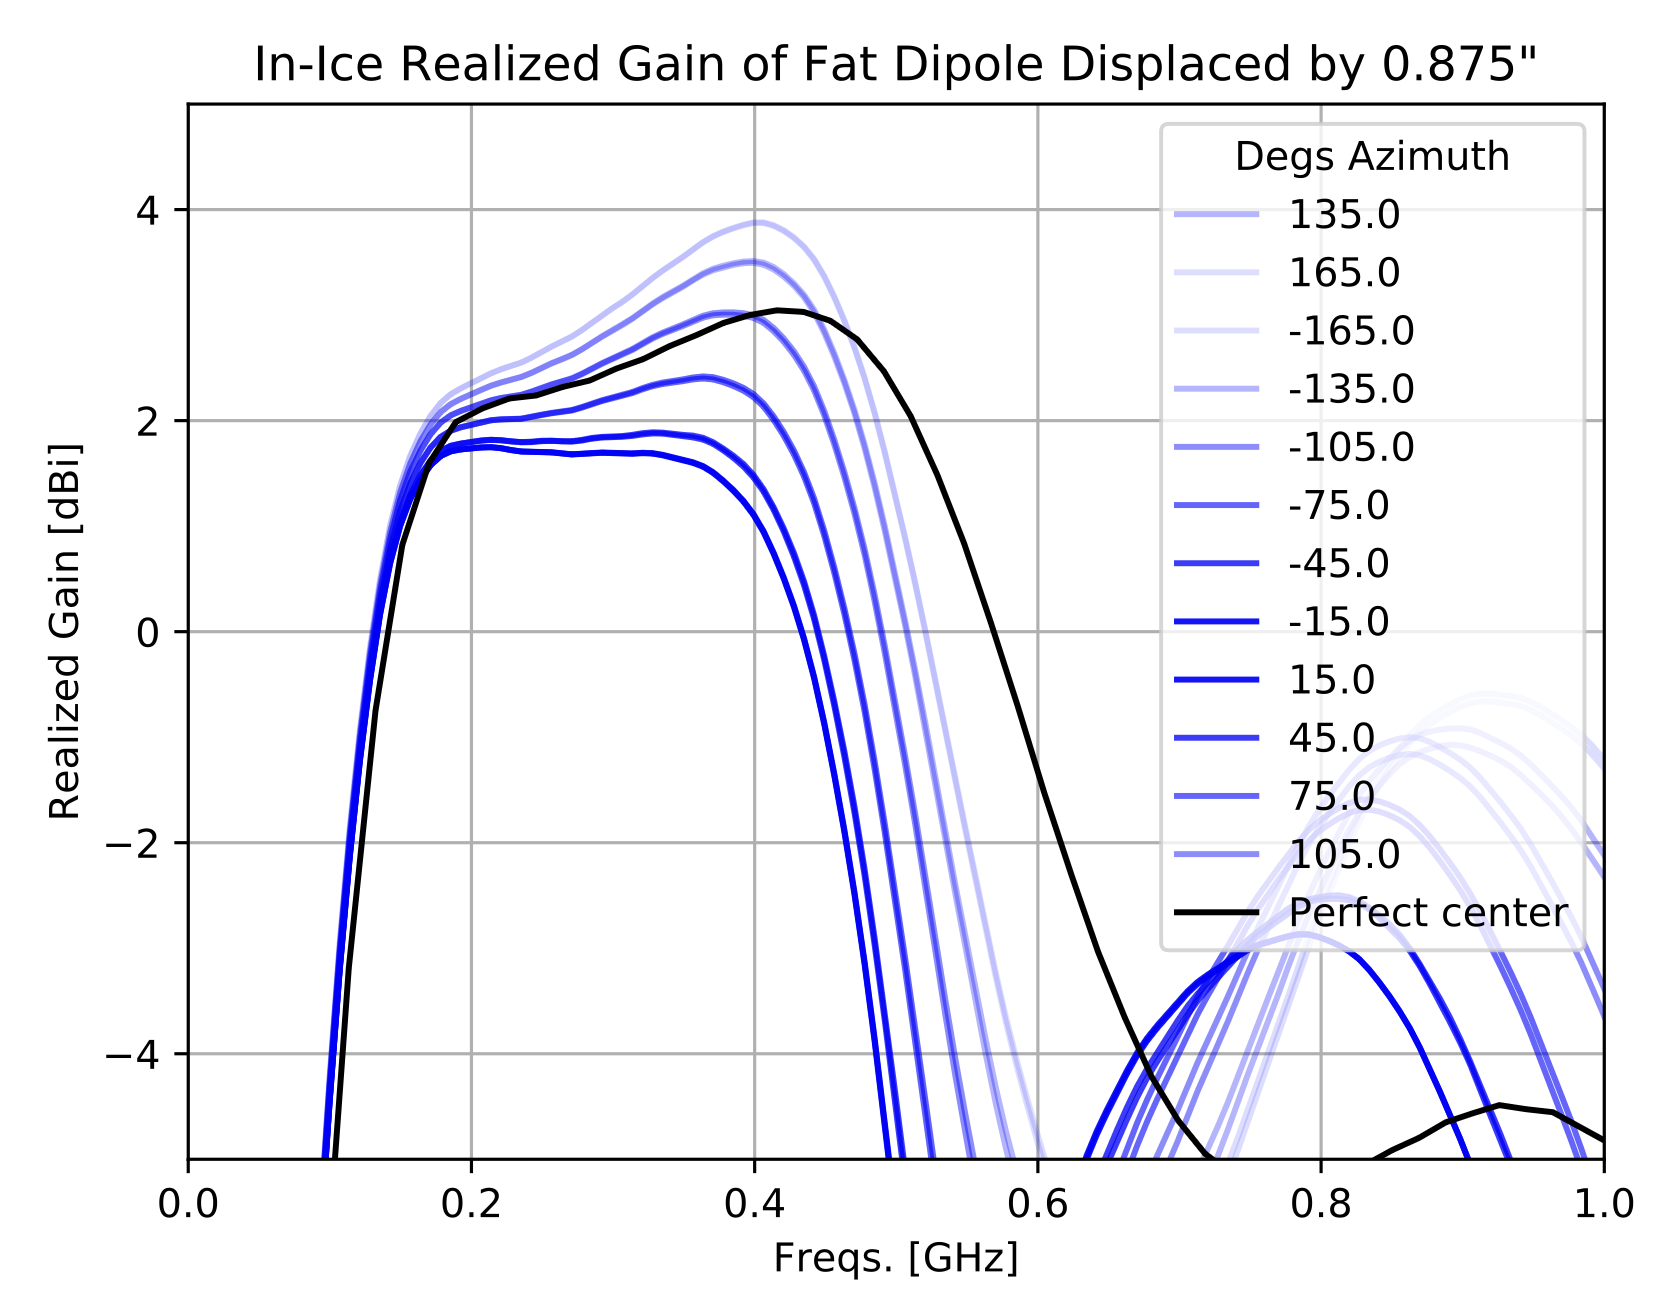
\includegraphics[
    width=0.7\textwidth,
    alt={}
  ]{sections/spacers/images/antenna_centering.png}
  \caption{
    Simulation of the realized gain of a vertically polarized antenna in a 5.75~inch diameter borehole displaced 0.875~inches in various directions in azimuth (blue lines).
    These can be compared the realized gain of a perfectly centered vertically polarized antenna (black line).
    Adapted from Ref.~\citep{thesis_dansmith}.
  }
  \label{fig:antenna_displacement}
\end{figure}

Jeff Cherwinka created the first design for the antenna centralizers and I completed testing and finalization of the design. 
Figure~\ref{fig:spacers_assembled} shows the computer animated design and a photo of a deployed centralizer on an \mbox{RNO-G} string. 
The centralizer is composed of two pieces of high density polyethylene cut with holes that fit push-in rivets and notches that fit around the rope that the string is deployed on.
When each piece of plastic is bent into a ring, its shape is secured with the push in rivets.
Two rings are then interlocked to create a sphere centered around the rope.
The final design for the plastic pieces is showed in Fig.~\ref{fig:spacers_cad}

\begin{figure}
  \centering
  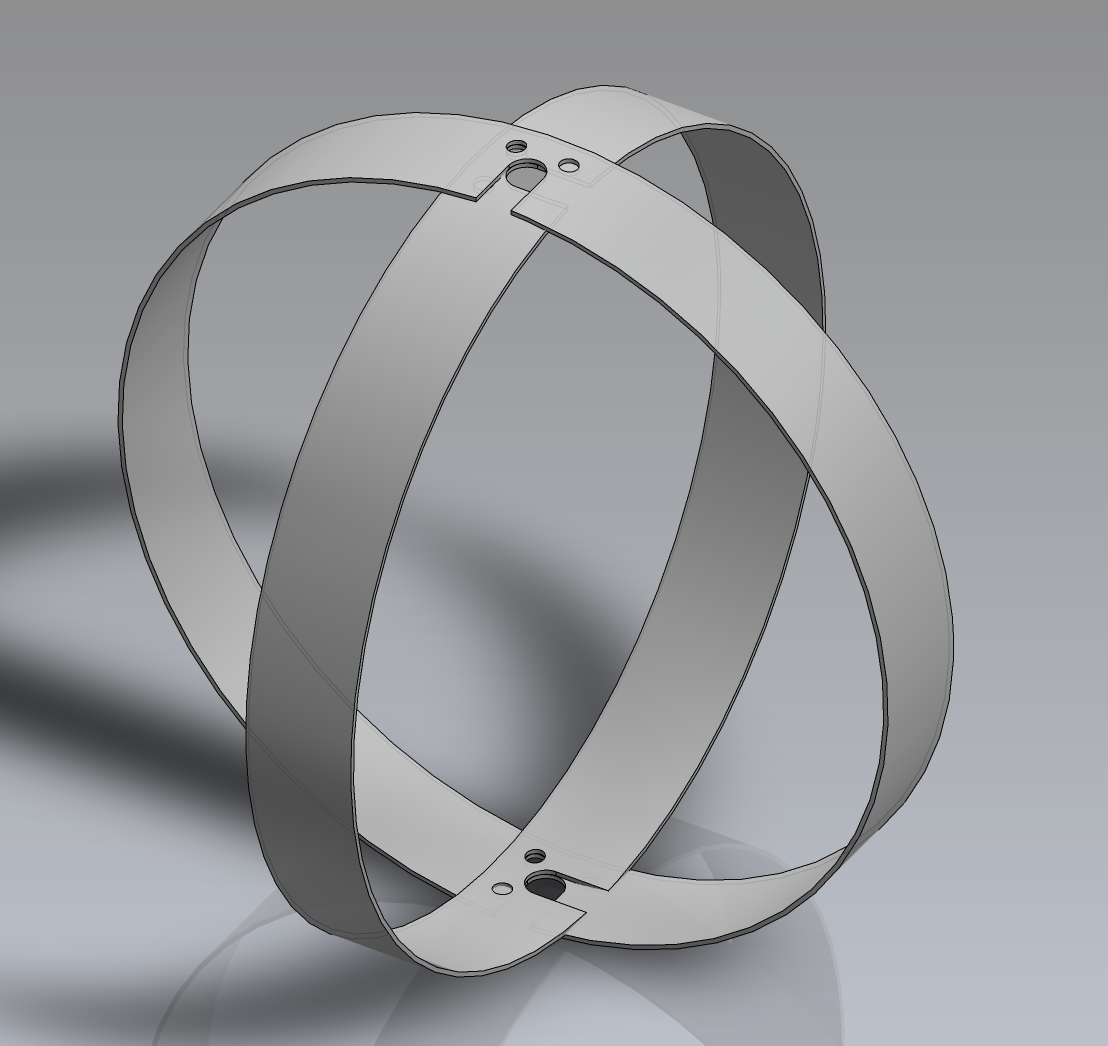
\includegraphics[
    width=0.5\textwidth,
    alt={}
  ]{sections/spacers/images/Assembled_spacer.png}
  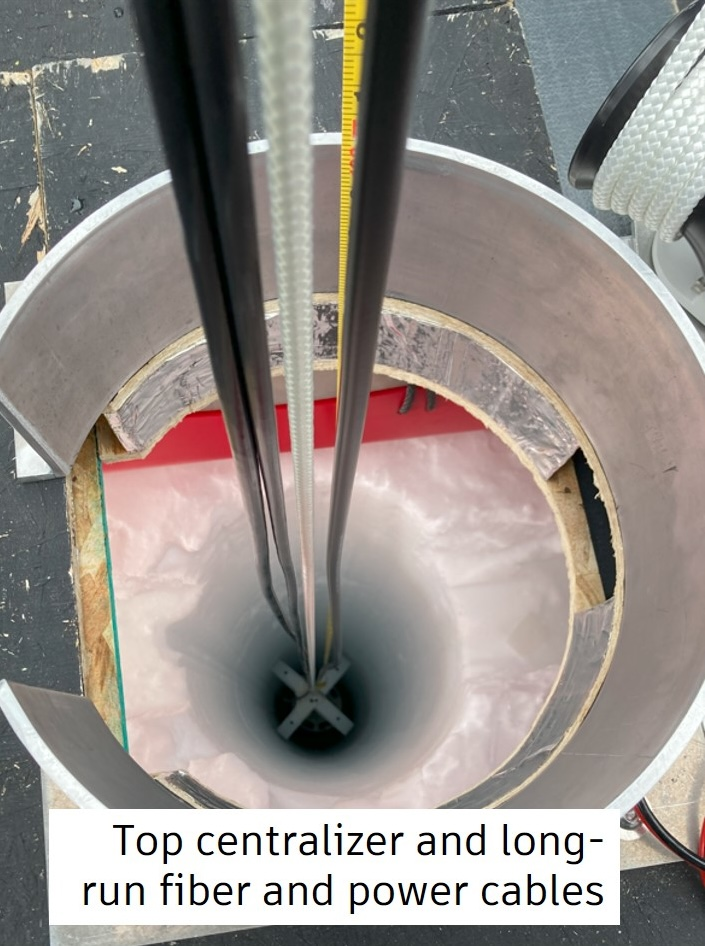
\includegraphics[
    width=0.4\textwidth,
    alt={}
  ]{sections/spacers/images/deployed_spacer.jpg}
  \caption{
    Left: Computer animated design showing the assembled version of a preliminary centralizer, courtesy of Jeff Cherwinka. 
    Right, a centralizer deployed down an \mbox{RNO-G} borehole.
  }
  \label{fig:spacers_assembled}
\end{figure}


\begin{figure}
  \centering
  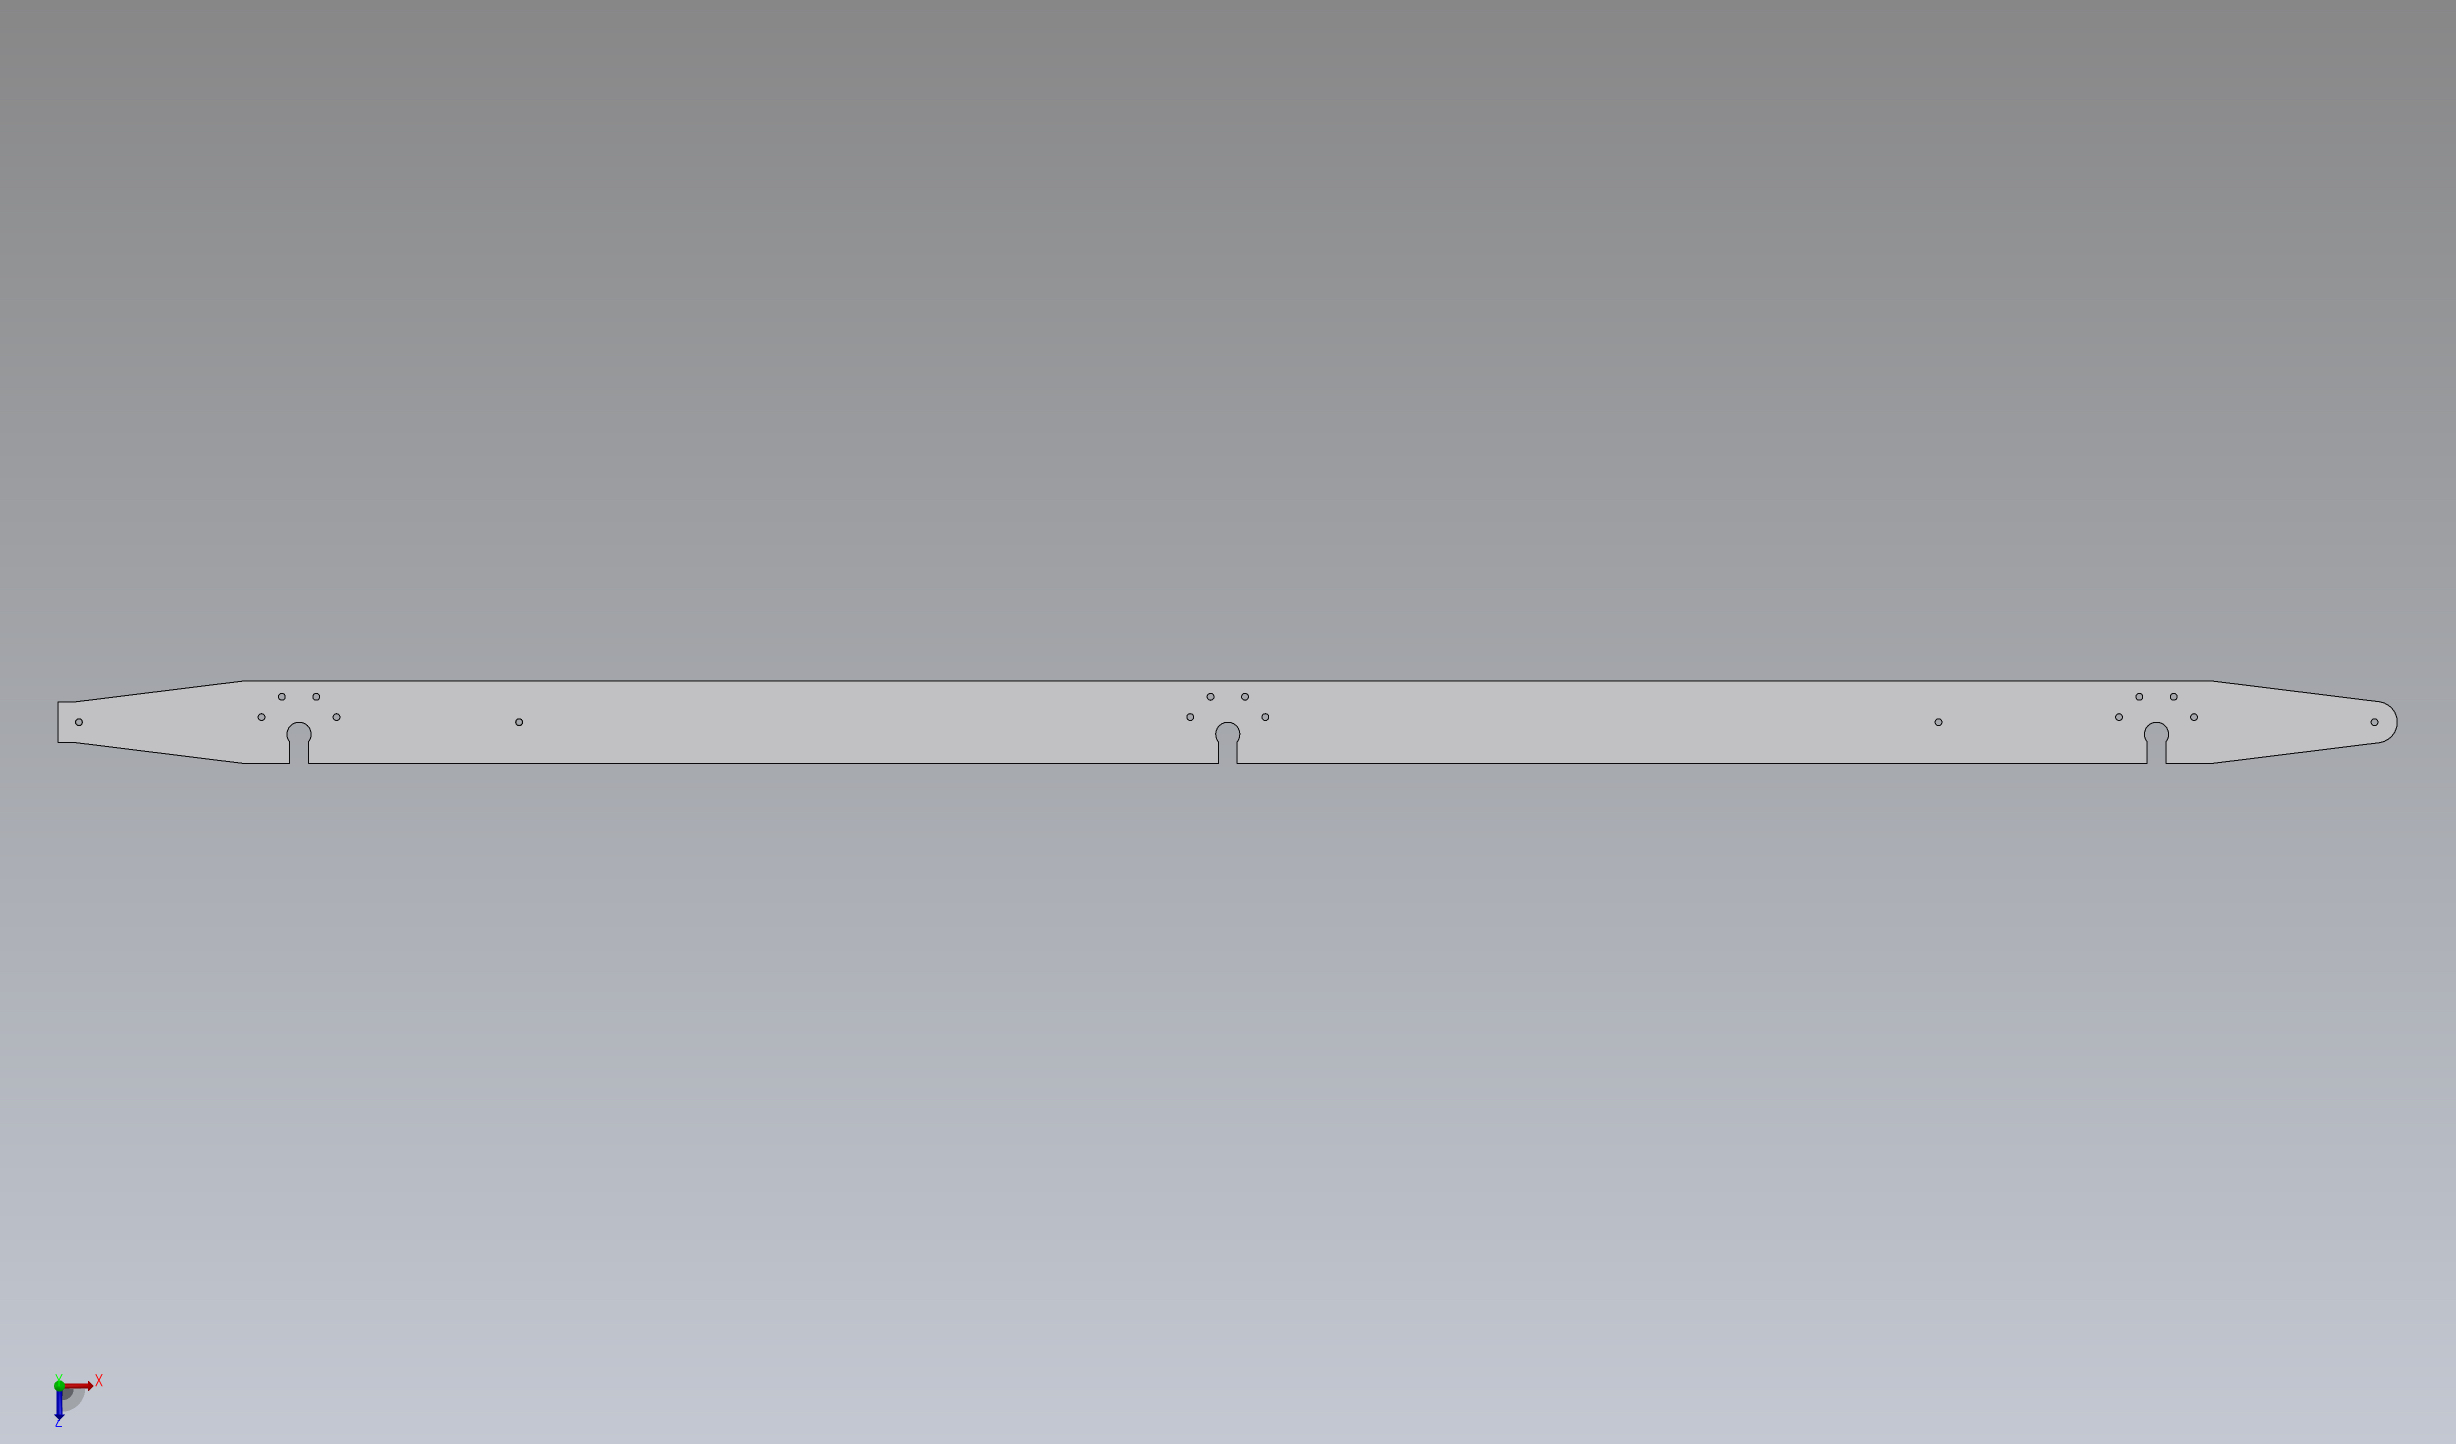
\includegraphics[
    width=\textwidth,
    alt={}
  ]{sections/spacers/images/Bishop-Flat_Spacer.jpg}
  \caption{
    Computer animated design showing one of two plastic sheets used to create the two interlocking rings that make up an \mbox{RNO-G} antenna centralizer.
  }
  \label{fig:spacers_cad}
\end{figure}

The centralizers are installed at the top of each antenna cluster on each \mbox{RNO-G} string shown in Fig.~\ref{fig:rnog}~\citep{rnog_initialperformance}.
This means there are 4 centralizers deployed on the power string and one centralizer on each helper string- six per \mbox{RNO-G} station.
Centralizers have been included in \mbox{RNO-G} stations deployed in 2022 and onwards.

% Theres a centralizer on page 5 of https://radio.uchicago.edu/wiki/images/6/68/\mbox{RNO-G}-2024-weeklyReport-July8-3.pdf